% Бүлэг 2

\chapter{Прокси дахин шифрлэлтэд суурилсан файл хуваалцах систем} % Зарим нэг зөвлөмж
\label{Chapter2} % Энэ бүлэг рүү ишлэл хийх бол \ref{Chapter2} командыг ашигла 
\pagecolor{white}

%-------------------------------------------------------------------------------
%	SECTION 1
%-------------------------------------------------------------------------------
\section{Прокси дахин шифрлэлт}
Прокси дахин шифрлэлт нь нийтийн түлхүүрээр шифрлэсэн өгөгдлийг дахин шифрлэж өөр хувийн түлхүүрээр тайлах боломжийг олгодог.

Мамбо болон Окамото шифрийг тайлан дараа нь шифрлэх уламжлалт аргыг сайжруулах зорилгоор анх гаргаж ирсэн.

1998 онд Blaze, Bleumer, Strauss (BBS) нар "atomic proxy cryptography" гэсэн ойлголтыг санал болгосон бөгөөд үүнд хагас итгэмжлэгдсэн прокси нь үндсэн энгийн текстийг харалгүйгээр Алисын шифрийг Бобын шифр текст болгон хувиргадаг. El Gamel дээр суурилсан схем ба прокси буюу гуравдагч талийн тусламжтайгаар шифрийг дамжуулах зорилготой. \cite{ateniese2005improved}

Прокси дахин шифрлэлт үйл явц нь гурван хэсгээс тогтоно.
\begin{itemize}
    \item \textbf{Төлөөлөгч:} Прокси дахин шифрлэлт ашиглан шифрийг тайлах эрхээ өөр хүнд шилжүүлэх өгөгдлийн эзэн. Дахин шифрлэлтийн түлхүүр үүсгэж, прокси руу илгээдэг. Төлөөлөгчийг ихэвчлэн “Алис” гэж нэрлэдэг.
    \item \textbf{Орлгоч:} Төлөөлөгчийн шифрийг тайлах эрхтэй хүн. Ихэвчлэн "Боб" гэдэг нэртэй байдаг.
    \item \textbf{Прокси:} Дахин шифрлэх шифрийг дамжуулах гуравдагч тал.
\end{itemize}

\textbf{Прокси дахин шифрлэлт үндсэн хоёр төрөлтэй.}
\begin{itemize}
    \item Нэг чиглэлт (Unidirectional PRE)
    \item Хоёр чиглэлт (Bidirectional PRE)
\end{itemize}
Мөн олон дахин шифрлэх боломжтой болон нэг л дахин шифрлэх боломжтой гэж хуваадаг.

Нэг чиглэлт \emph{PRE (KE, RG, E, R, D)} хэсгүүдээс тогтоно.
\begin{enumerate}
    \item Алис, Боб болон Чарли хувийн болон нийтийн түлхүүрийг үүсгэнэ. \emph{(KE)}
    \item Алис Боб-д зориулж өгөгдлөө шифрлэж серверт байршуулна.
    \item Боб Алис-ын өгөгдлийг Чарли-тай хуваацлахын тулд \emph{RE(pkB,skB,pkC,skC∗)} шифрлэж серверт байршуулна. Чарлигийн хувийн заавал шаардахгүй үүсгэж болно.
    \item Боб RE-г ашиглаж үүсгэсэн түлхүүрийг серверт явуулж Алисын файлыг дахин шифрлэж Чарли тайлах боломжтой болно.
\end{enumerate}

\begin{figure}[ht]
\centering
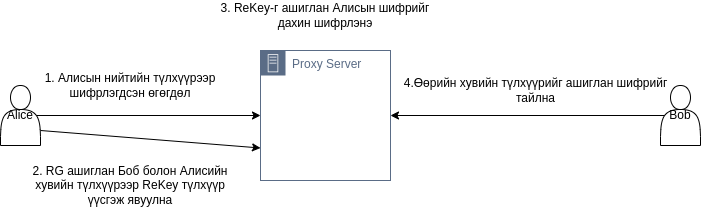
\includegraphics[scale=0.5]{Figures/PRE.drawio.png}
\caption[Proxy Re-encryption scheme]{Прокси дахин шифрлэх}
\label{fig:PRE_Scheme}
\end{figure}

Давуу талууд:
\begin{itemize}
    \item Нууцлалыг сайжруулна: PRE нь оролцогч талуудын хувийн мэдээллийг задруулахгүйгээр өгөгдлийг хуваалцахыг зөвшөөрснөөр нууцлалыг сайжруулдаг. Талууд нууцаар эсвэл хувийн нууц мэдээллийг задруулахгүйгээр мэдээллээ хуваалцахыг хүссэн тохиолдолд ашиглах боломжтой.
    \item Илүү уян хатан шифрлэсэн өгөгдлийг өргөн хүрээтэй тараах боломжтой
\end{itemize}

Сул талууд:
\begin{itemize}
    \item Проксид итгэх: PRE нь дахин шифрлэлтийг гүйцэтгэхэд гуравдагч талын прокси дээр тулгуурладаг ба схемийн аюулгүй байдал нь прокси талаас хамаарна.
    \item Хязгаарлагдмал өргөтгөх чадвар: PRE нь өргөтгөх чадварын хувьд хязгаарлагдмал байж болно. Учир нь хэрэглэгчдийн тоо нэмэгдэхийн хэрээр олон талыг дэмжихэд шаардлагатай дахин шифрлэлтийн түлхүүрүүдийн тоо хурдацтай өсөх болно. Энэ нь гол менежментийг төвөгтэй болгож, удирдахад хэцүү болгодог.
    \item Potential for replay attacks: PRE нь халдагч хариуг зогсоож хандах эрхийг өөрт ашигтай солих боломжтой. 
    \item Хүчингүй болгоход хүндрэлтэй: PRE дахь өгөгдөлд хандах эрхийг цуцлах нь ялангуяа олон тал оролцсон тохиолдолд төвөгтэй. Хэрэв аль нэг талын дахин шифрлэлтийн түлхүүр алдагдсан бол бусад талуудын мэдээлэлд хандах эрхэд нөлөөлөхгүйгээр өгөгдөлд хандах эрхийг цуцлах нь хэцүү юм.
    \item Хязгаарлагдмал хэрэглээ: PRE нь харьцангуй шинэ бөгөөд шинээр гарч ирж буй технологи хэвээр байгаа бөгөөд илүү уламжлалт шифрлэлтийн схемүүдтэй харьцуулахад хэрэглээ нь хязгаарлагдмал байдаг. Энэ нь технологийг хэрэгжүүлэх, удирдах туршлагатай мэргэжилтнүүд бага байдаг.
\end{itemize}

\subsection*{Прокси дахин шифрлэх схемийн ерөнхий хэрэглээ}
\begin{itemize}
    \item \textbf{Аюулгүй өгөгдөл хуваалцах:} Өгөгдлийн олон хэрлэгчид найдвартай хуваалцахад ашигладаг. Өгөгдлийн эзэмшигч нь өгөгдлийг өөрийн түлхүүрээр шифрлэж, дахин шифрлэж прокси руу шилжүүлдэг. Дараа нь прокси нь хүлээн авагчийн түлхүүрээр шифрлэгдсэн өгөгдлийг хувиргаж, өгөгдөл эзэмшигчийн оролцоогүйгээр шифрийг тайлж, өгөгдөлд хандах боломжийг олгодог.

    \item \textbf{Cloud Storage:} Үүл хадгалах системд хадгалагдсан мэдээллийн аюулгүй байдлыг сайжруулахын тулд прокси дахин шифрлэлтийг ашиглаж болно. Нууц мэдээллийг үүлэн үйлчилгээ үзүүлэгч рүү шууд оруулахын оронд өгөгдлийг эзэмшигчийн түлхүүрээр шифрлэж, прокси түлхүүрээр дахин шифрлэх боломжтой. Дараа нь прокси нь дахин шифрлэгдсэн өгөгдлийг үүлэн дотор хадгалдаг. Энэ нь үүлэн үйлчилгээ үзүүлэгч нь зөвхөн дахин шифрлэгдсэн өгөгдөлд хандах эрхтэй бөгөөд анхны контентыг уншиж чадахгүй байх боломжийг олгодог.

    \item \textbf{Түлхүүр эскроу:}Түлхүүр эскроу гэдэг нь криптограф түлхүүрийг итгэмжлэгдсэн гуравдагч этгээдэд хадгалах практикийг хэлнэ. Энэ тохиолдолд анхны өгөгдөл нь эзэмшигчийн түлхүүрээр шифрлэгдсэн бөгөөд дахин шифрлэлтийн түлхүүрnийг проксид хадгалагдана. Хэрэв эзэмшигч нь түлхүүрээ алдсан эсвэл өөр төхөөрөмжөөс хандах шаардлагатай бол прокси нь өгөгдлийг шинэ түлхүүрээр дахин шифрлэх боломжтой бөгөөд ингэснээр эзэмшигчид дахин хандах эрх олгоно.

    \item \textbf{Аюулгүй Имэйл Холбоо:} Илгээгч нь хувийн түлхүүрээ шуудангийн сервер эсвэл бусад зуучлагчтай хуваалцахын оронд өөрийн түлхүүрээр имэйлээ шифрлэж, дахин шифрлэх ажиллагааг прокси руу шилжүүлэх боломжтой. Дараа нь прокси нь хүлээн авагчийн түлхүүрээр имэйлийг дахин шифрлэх боломжтой бөгөөд зөвхөн хүлээн авагч нь мессежний кодыг тайлж унших боломжтой.
\end{itemize}
% \subsection*{Прокси дахин шифрлэх схемийн ашиглаж буй системүүд}
% \begin{itemize}
%     \item Google Cloud Platform (GCP) Cloud Түлхүүр Удирдлагын Үйлчилгээ: GCP Үүлэн Түлхүүр Удирдлагын Үйлчилгээ нь үүлэнд суурилсан программууд, гар утасны программууд болон вэб программууд зэрэг төрөл бүрийн программуудын шифрлэлтийн түлхүүрүүдийг хадгалахад ашиглагдаж болно. PRE нь хэрэглэгчдэд шифрлэлтийн түлхүүрийг хуваалцах шаардлагагүйгээр шифрлэгдсэн өгөгдлийг бусадтай хуваалцах боломжийг олгоход ашиглаж болно. Жишээлбэл, компани GCP Cloud Түлхүүр Удирдлагын Үйлчилгээг ашиглан үйлчлүүлэгчийнхээ мэдээллийн шифрлэлтийн түлхүүрүүдийг хадгалах боломжтой. Дараа нь компани PRE-г ашиглан ажилтнууддаа шифрлэлтийн түлхүүрүүдийг ажилчидтайгаа хуваалцахгүйгээр хэрэглэгчийн мэдээлэлд хандах боломжийг олгох боломжтой. Энэ нь ажилтны компьютер эвдэрсэн ч гэсэн хэрэглэгчийн мэдээллийн нууцлалыг хамгаалахад тусална.
% \end{itemize}

%-------------------------------------------------------------------------------
%	SECTION 2
%-------------------------------------------------------------------------------
\section{Хөгжүүлэх технологи, хэл сонгох}
Прокси дахин шифрлэлт файл хуваалцах системийг хөгжүүлэхэд ашиглах технологийн судалгаа хийсэн.
Систем хоёр хэсгээс тогтох ба. API сервер болон хэрлэгч талын программ. Пайтон маш олон нэмэлт сангууд байдаг маш том нийгэмлэгтэй (community) хэл. Бичиглэл хялбар олон давуу талтай тул пайтон хэлийг сонгосон.
Үүнд:
\begin{itemize}
    \item \textbf{Flask}\\
    Пайтон хэл дээр бичсэн веб хөгжүүлэхэд зориулагдсан фреймворк юм. Хөнгөхөн олон сан шаардахгүй. Сурахад хялбар өөрийн хүссэн загвараар загварчилж хийх боломжтой. RESTFul API гаргахад хялбар. Хэрэгтэй гэвэл нэмэлт сан ORM зэрэг өөр сангууд суулгаж хамт ашиглах боломжтой.
    \item \textbf{Tkinter}\\
    Хэрэглэгчийн интерфейс (GUI) үүсгэхэд ашигладаг Python номын сан юм. Tcl/TK GUI дээр суурилсан. Линукс виндовс зэрэг олон үйлдлийн системийг дэмждэг. Нэмэлт сангуудтай ажиллах боломжтой.
    \item \textbf{pyUmbral}\\
    Прокси дахин шифрлэлтийг файтон дээр хэрэгжүүлсэн пайтоны сан юм. OpenSSL болон Cryptography.io ашиглсан.
    \item \textbf{Google Cloud Platform}\\
    Гуравдагч тал болох сервер проксиг (API) deploy хийж байршуулах шаардлагатай0. Google Cloud нь маш олон давуу талтай ба үнэгүй туршиж үзэх 300 долларын эрхтэй тул сонгосон.
\end{itemize}

%-------------------------------------------------------------------------------
%	SECTION 3
%-------------------------------------------------------------------------------
\section{Хөгжүүлэлтийн орчин бэлдэх}
Пайтон хэл нь орчин бүрдүүлэхэд хялбар ба виртуал орчин үүсгэж хэрэгтэй сангуудыг татаж суулгах боломжтой. Бүх линукс тархцад пайтон хэл нь суулгалцан байдаг тул хэрэгтэй сангуудыг татаж суулгахад л хангалтай.

Прокси дахин шифрлэлт сан пайтон дээр сан бичих гэж оролдсон. JHU-MTI Прокси дахин шифрлэлтийн сан нь C/C++ хэл дээр бичигдсэн байсан. Пайтон хэлний setuptools болон C хэлний "python.h" санг ашиглан пайтоны сан бичих гэж оролдож үзсэн. JHU-MTI сан нь MIRCL санг ашигладаг.
\\
\textbf{Ерөнхий бүтэц}
\dirtree{%
.1 ..
.2 example.
.3 example.py.
.2 external.
.3 miracl.
.3 proxylib.
.2 LICENSE.
.2 README.md.
.2 setup.py.
.2 src.
.3 pypre.cpp.
.2 userguide.pdf.
}

Илүү үр дүнтэй хурдан хийхийн тулд pyUmbral санг сонгож ашигласан.

%-------------------------------------------------------------------------------
%	SECTION 4
%-------------------------------------------------------------------------------
\section{Бүлгийн дүгнэлт}
Прокси дахин шифрлэлт судлаж системийг хөгжүүлэлтэнд шаардлагатай технологиуд сангуудыг судлаж хөгжүүлэлт хийж эхэлсэн.